\documentclass[border=2pt]{standalone}
\usepackage{tikz}
\usepackage{amsmath}
\usepackage{mathtools}
\usepackage{adjustbox}
\usetikzlibrary{patterns}
\usetikzlibrary{calc} \usetikzlibrary{positioning} \usetikzlibrary{shapes,arrows} \usetikzlibrary{plotmarks}
\usetikzlibrary{positioning,decorations.pathreplacing}

\begin{document}

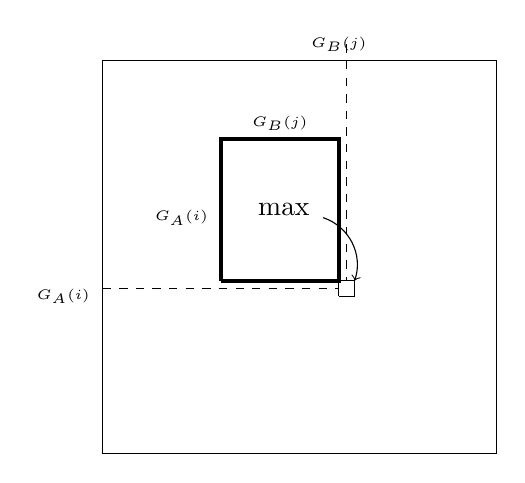
\begin{tikzpicture}
\draw (0,0) -- (5,0) -- (5,5) -- (0,5) -- (0,0);
\draw (3,2) -- (3.2,2) -- (3.2,2.2) -- (3,2.2) -- (3,2);

\node[] at (-0.5, 2) {\tiny $G_A(i)$};
\node[] at (3, 5.2) {\tiny $G_B(j)$};

\draw[line width=0.5mm] (1.5, 2.2) -- (3,2.2) -- (3, 4) -- (1.5, 4) -- (1.5, 2.2);

\node[] at (1, 3) {\tiny $G_A(i)$};
\node[] at (2.25, 4.2) {\tiny $G_B(j)$};

\draw[dashed] (0, 2.1) -- (3, 2.1);
\draw[dashed] (3.1, 5.2) -- (3.1, 2.2);

\node[] at (2.3, 3.1) {$\max$};

\path[solid,->](2.8, 3) edge [bend left=45]  (3.2, 2.2);

\end{tikzpicture}

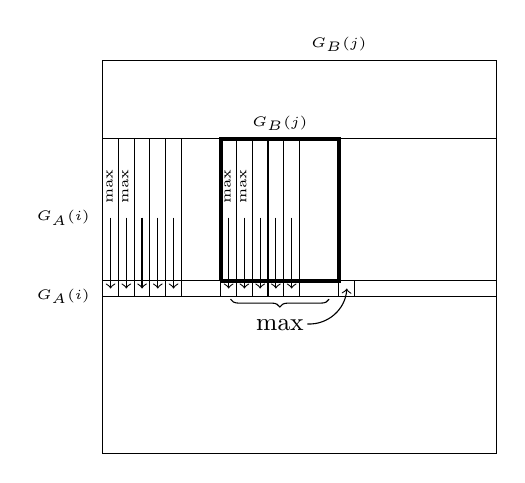
\begin{tikzpicture}
\draw (0,0) -- (5,0) -- (5,5) -- (0,5) -- (0,0);
\draw (3,2) -- (3.2,2) -- (3.2,2.2) -- (3,2.2) -- (3,2);

\node[] at (-0.5, 2) {\tiny $G_A(i)$};
\node[] at (3, 5.2) {\tiny $G_B(j)$};

\draw[line width=0.5mm] (1.5, 2.2) -- (3,2.2) -- (3, 4) -- (1.5, 4) -- (1.5, 2.2);

% horizontal 
\draw (0, 2.2) -- (5, 2.2);
\draw (0, 2) -- (5, 2);
\draw (0, 4) -- (5, 4);

% vertical
\draw (0.2, 2) -- (0.2, 4);
\draw (0.4, 2) -- (0.4, 4);
\draw (0.6, 2) -- (0.6, 4);
\draw (0.8, 2) -- (0.8, 4);
\draw (1.0, 2) -- (1.0, 4);
  % our area
\draw[line width=0.1mm] (1.5, 2) -- (1.5, 4);
\draw (1.7, 2) -- (1.7, 4);
\draw (1.9, 2) -- (1.9, 4);
\draw (2.1, 2) -- (2.1, 4);
\draw (2.3, 2) -- (2.3, 4);
\draw (2.5, 2) -- (2.5, 4);

% vertical max
\path[solid,->](0.1, 3) edge node[above right=5mm and 1.5mm, rotate=90]{\tiny $\max$}  (0.1, 2.1);
\path[solid,->](0.3, 3) edge node[above right=5mm and 1.5mm, rotate=90]{\tiny $\max$} (0.3, 2.1);
\path[solid,->](0.5, 3) edge  (0.5, 2.1);
\path[solid,->](0.7, 3) edge  (0.7, 2.1);
\path[solid,->](0.9, 3) edge  (0.9, 2.1);
  % our area
\path[solid,->](1.6, 3) edge node[above right=5mm and 1.5mm, rotate=90]{\tiny $\max$} (1.6, 2.1);
\path[solid,->](1.8, 3) edge node[above right=5mm and 1.5mm, rotate=90]{\tiny $\max$} (1.8, 2.1);
\path[solid,->](2.0, 3) edge  (2.0, 2.1);
\path[solid,->](2.2, 3) edge  (2.2, 2.1);
\path[solid,->](2.4, 3) edge  (2.4, 2.1);

\node[] at (-0.5, 3) {\tiny $G_A(i)$};
\node[] at (2.25, 4.2) {\tiny $G_B(j)$};

%\draw[dashed] (0, 2.1) -- (3, 2.1);
%\draw[dashed] (3.1, 5.2) -- (3.1, 2.2);

% \node[] at (2.3, 3.1) {${\tt MAX}$};

\node[](start) at (1.5, 2.0) {};
\node[](end) at (3, 2.0) {};

\draw[decorate,decoration={brace,amplitude=1mm, raise=1pt, mirror}](start)--node[black,midway,below=5pt] {\small $\max$}(end);

\path[solid,->](2.6, 1.65) edge [bend right=45]  (3.1, 2.1);

\end{tikzpicture}

\end{document}